% \newpage
% \begin{center}
% \normalfont\Large\bfseries MPC exercise: week three
% \end{center}
\setcounter{section}{0}

\section{Convex optimization}
Consider the optimization problem 
\begin{align*}
    \min_{x_1,x_2} \quad&f(x_1,x_2),\\
    \text{s.t.} \quad&2x_1 +x_2 \leq 1,\\
    &x_1 + 3x_2 \leq 1,\\
    &x_1\geq 0, x_2 \geq 0.
\end{align*}
Make a sketch of the feasible set. For each of the following objective functions, give the optimal set and the optimal value (adapted from Exercise 4.1 in Convex Optimization by Stephen Boyd and Lieven Vandenberghe).
\begin{enumerate}
    \item $f(x_1,x_2) = x_1 + x_2$.
    \item $f(x_1,x_2) = -x_1 - x_2$.
    \item $f(x_1,x_2) = x_1 $.
    \item $f(x_1,x_2) = \text{max}\{x_1,x_2\}$.
    \item $f(x_1,x_2) = x_1^2 + 9x_2^2$.
\end{enumerate}

\solution{See the Fig. \ref{ex3}
\begin{figure}[htbp]
    \centering
    \begin{minipage}{0.25\textwidth}
        \centering
        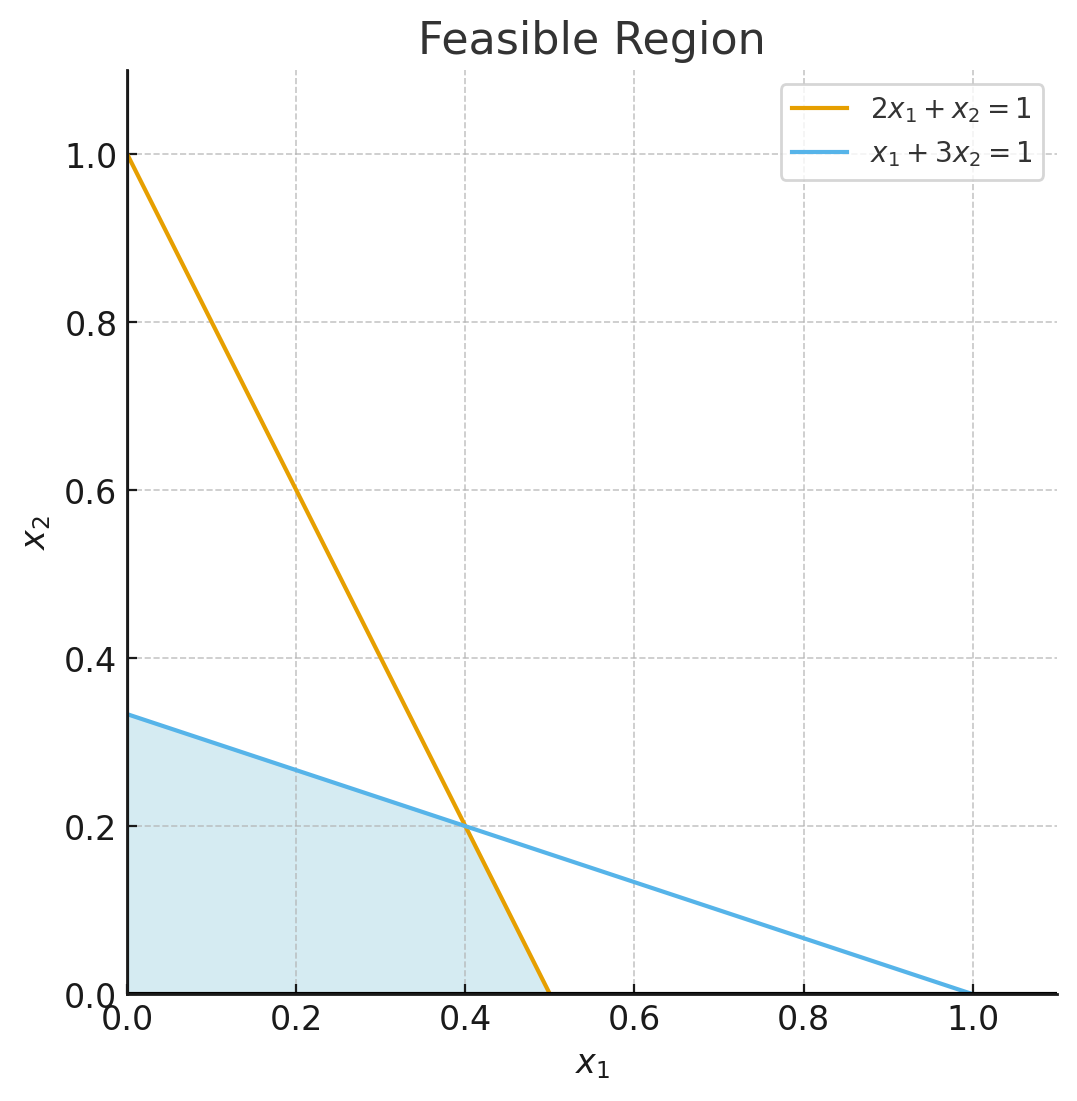
\includegraphics[width=\linewidth]{fig/feasible region.png}
        \caption*{Feasible region.}
    \end{minipage}\hfill
    \begin{minipage}{0.25\textwidth}
        \centering
        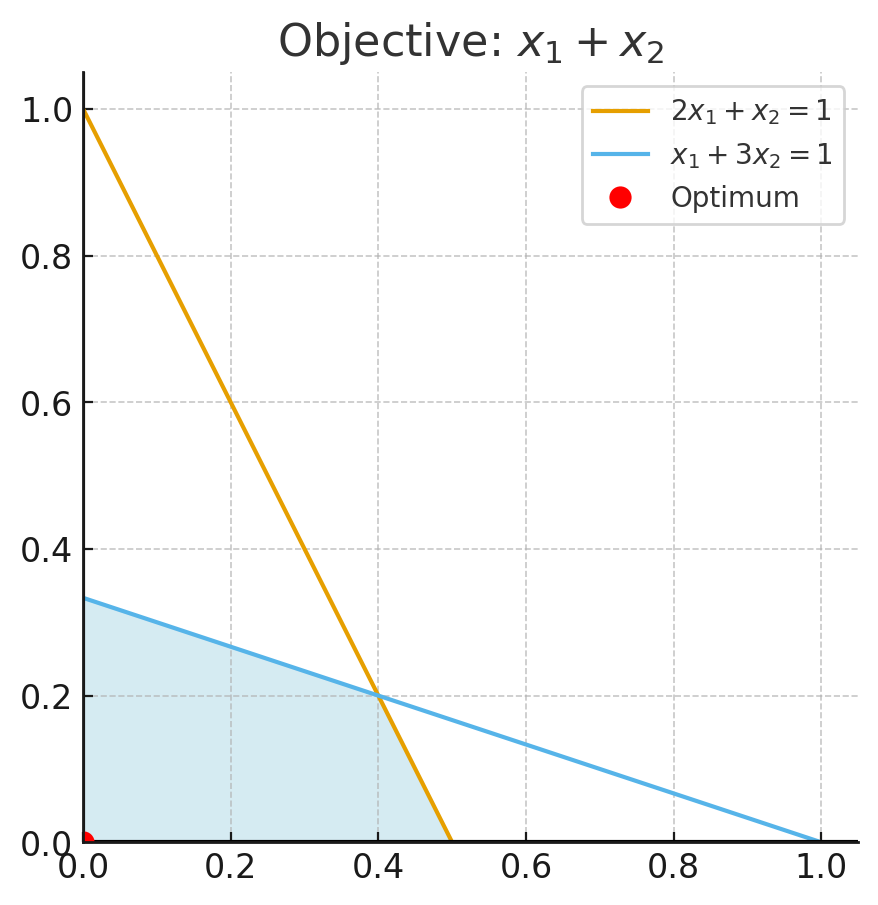
\includegraphics[width=\linewidth]{fig/1.png}
        \caption*{Objective 1.}
    \end{minipage}\hfill
    \begin{minipage}{0.25\textwidth}
        \centering
        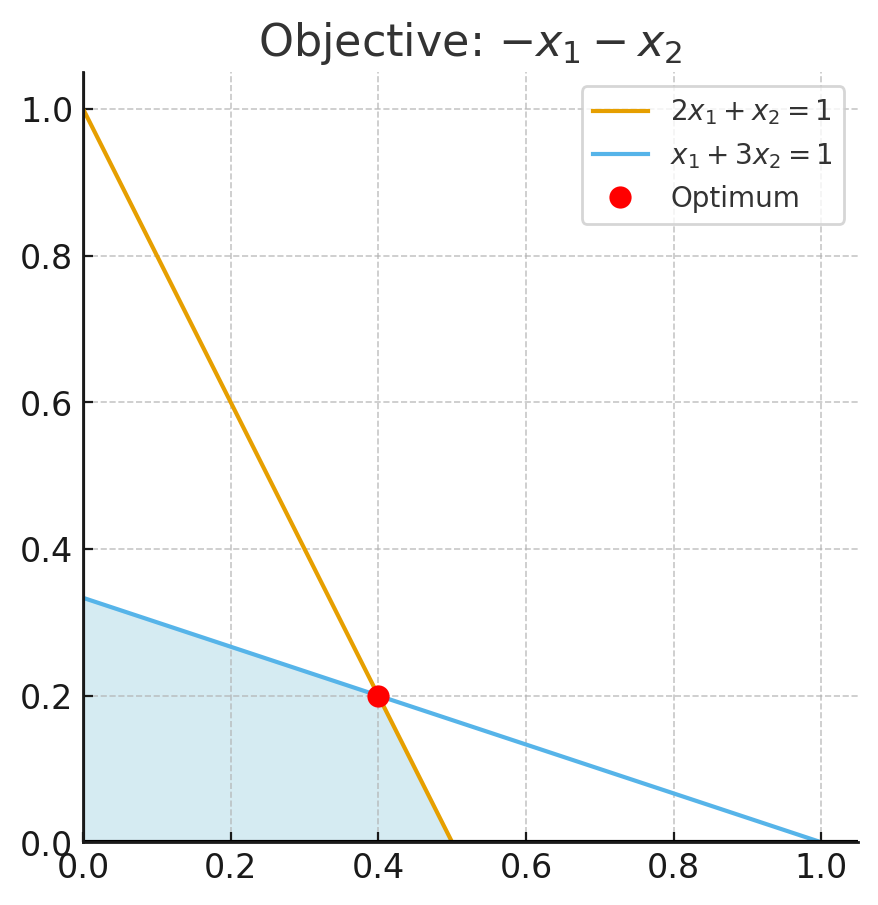
\includegraphics[width=\linewidth]{fig/2.png}
        \caption*{Objective 2.}
    \end{minipage}
    \vspace{0.3cm}
    \begin{minipage}{0.25\textwidth}
        \centering
        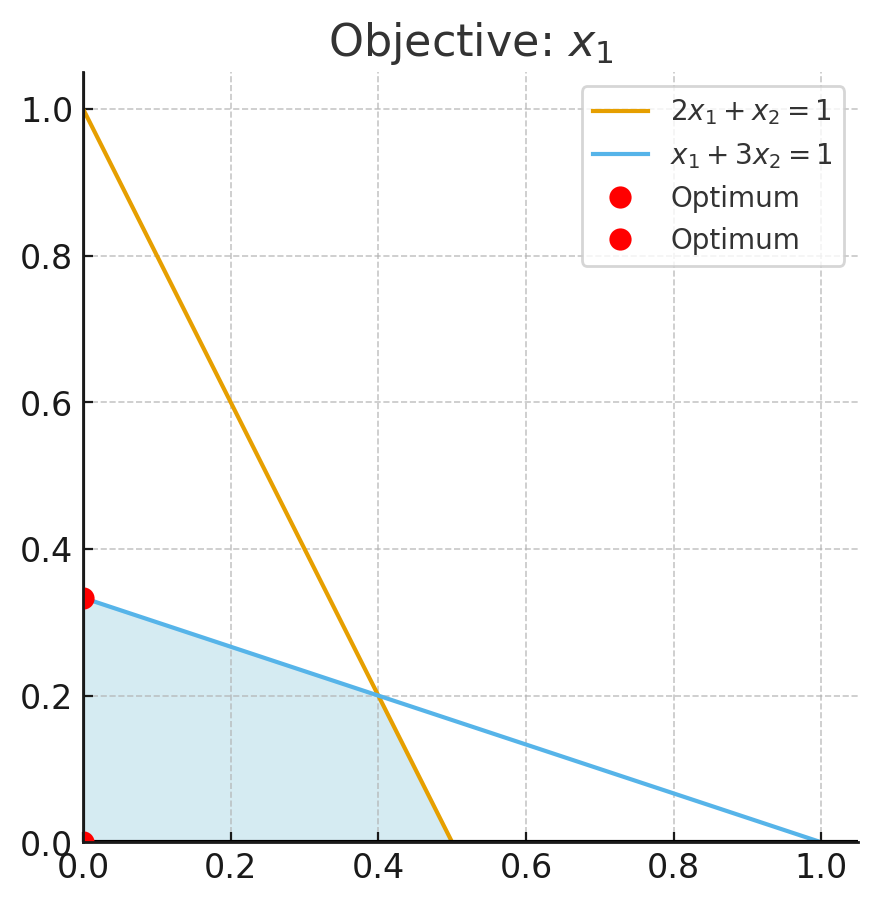
\includegraphics[width=\linewidth]{fig/3.png}
        \caption*{Objective 3.}
    \end{minipage}\hfill
    \begin{minipage}{0.25\textwidth}
        \centering
        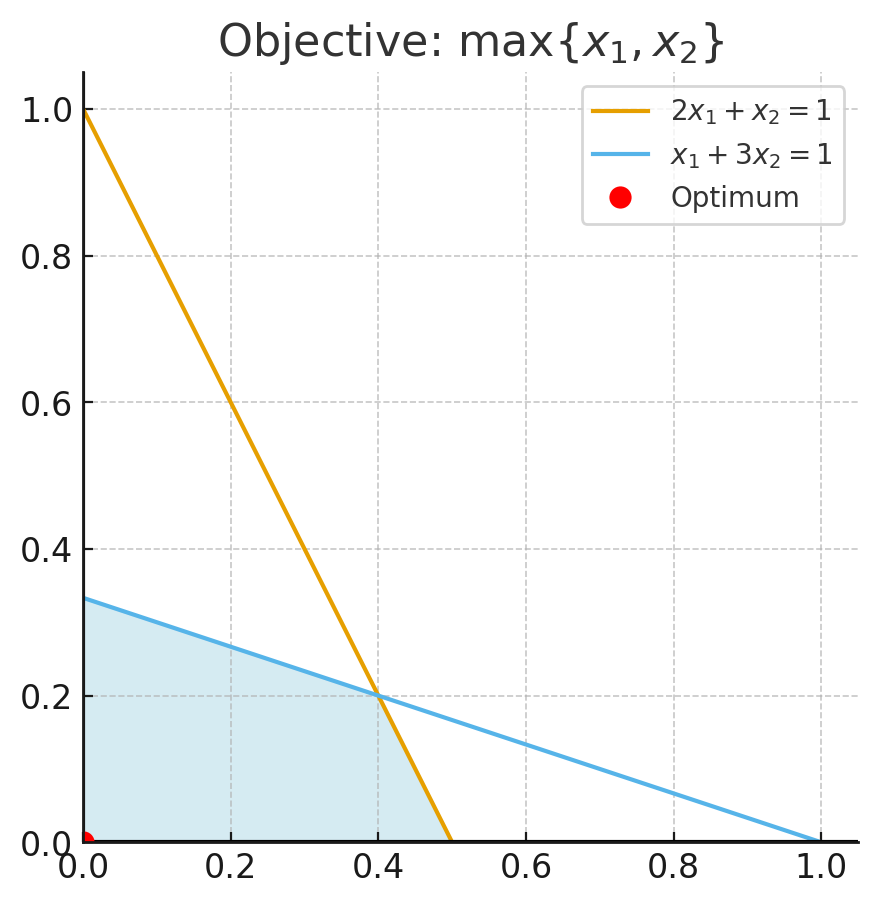
\includegraphics[width=\linewidth]{fig/4.png}
        \caption*{Objective 4.}
    \end{minipage}\hfill
    \begin{minipage}{0.25\textwidth}
        \centering
        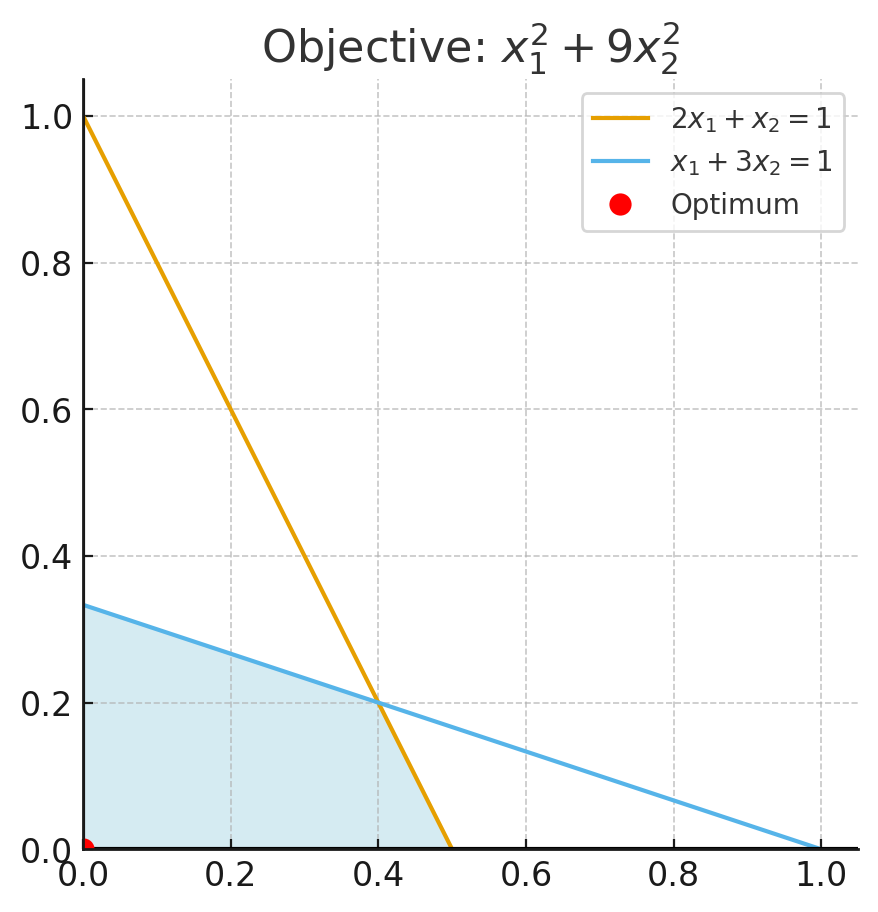
\includegraphics[width=\linewidth]{fig/5.png}
        \caption*{Objective 5.}
    \end{minipage}
    \caption{Solution of problem one.}
    \label{ex3}
\end{figure}}

\section{Logarithmic barrier interior-point method}
Consider the following Quadratically Constrained Quadratic Program (QCQP)
\begin{align*}
    \min_x \quad &x^{\top}Ax + c^{\top}x,\\
    \text{s.t.}\quad& x^{\top}Bx\leq\alpha,
\end{align*}

\begin{enumerate}
    \item Give the conditions on $B$ and $\alpha$ such that the problem always has an optimal solution. Describe the feasible set if these conditions are satisfied.

    \solution{If $B$ is positive definite, i.e., $B\succ 0$, and $\alpha\geq0$, the problem will always have a solution. Since in this case the feasible set is compact (bounded and closed), and $x^{\top}Ax+c^{\top}x$ is bounded from below on a compact set. The feasible set is an ellipsoid.}
    \item If both $A$ and $B$ are symmetric, write down the augmented objective function for the logarithmic barrier interior-point method.

    \solution{$f(x) = x^{\top}Ax + c^{\top}x - \kappa\log(-x^{\top}Bx+\alpha)$}
    \item Calculate the gradient and Hessian of the augmented objective function. 

    \solution{Gradient: $ \nabla f(x)  = 2Ax + c+\frac{2\kappa Bx}{\alpha - x^{\top}Bx}$.\\
    Hessian: $\nabla^2 f(x)  = 2A + \frac{2\kappa B(\alpha - x^{\top}Bx) + 4\kappa Bx(Bx)^{\top}}{(\alpha - x^{\top}Bx)^2}$}
    \item Assume that $A$ is positive definite, compute the Newton search direction, and prove that it is a descent direction if your condition given in 1 is satisfied.

    \solution{If $d$ is a descent direction, $\nabla f(x)^{\top}d\leq0$. We need to check if our Newton direction satisfies this condition.\\
    Newton direction: $d = -(\nabla^2f(x))^{-1}\nabla f(x) = -\big(2A + \frac{2\kappa B(\alpha - x^{\top}Bx) + 4\kappa Bx(Bx)^{\top}}{(\alpha - x^{\top}Bx)^2}\big)^{-1}\big(2Ax + c+\frac{2\kappa Bx}{\alpha - x^{\top}Bx}\big)$.\\
    Since $A$ is positive definite, $\big(2A + \frac{2\kappa B(\alpha - x^{\top}Bx) + 4\kappa Bx(Bx)^{\top}}{(\alpha - x^{\top}Bx)^2}\big)^{-1}$ is also positive definite. Hence $y^{\top}(\nabla^2 f(x))^{-1}y\geq0,\forall y.$ This means for the Newton direction $d$, $\nabla f(x)^{\top}d\leq0$. This shows that $d$ is indeed a descent direction.}
\end{enumerate}